\newif\ifstandalone
\standalonetrue % comment out for compilation with ktikz

\ifstandalone
\documentclass{standalone}
\fi

\usetikzlibrary{arrows,positioning, shapes.geometric}
\def\layersep{0.65cm}
\def\xconnection (#1,#2) {\draw[connection] (#1.north west) -- (#2.south east);  \draw[connection] (#1.north east) -- (#2.south west);}
\def\connection (#1,#2) {\draw[connection] (#1.north west) -- (#2.south west);  \draw[connection] (#1.north east) -- (#2.south east);}

\ifstandalone
\begin{document}
\fi

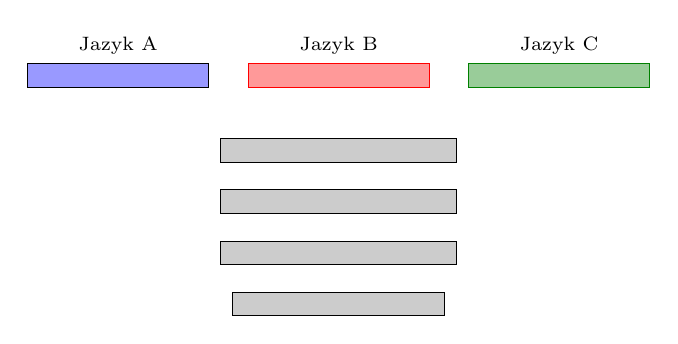
\begin{tikzpicture}[draw=black, node distance=\layersep, every node/.style = {font=\scriptsize}]
	   
 \tikzstyle{layer}=[rectangle, draw=black, fill=gray!40, minimum height=0.3cm, line width=0cm]
	\tikzstyle{hidden layer}=[layer, minimum width=3cm]
	\tikzstyle{input layer}=[layer, minimum width=2.7cm]
	\tikzstyle{output layer}=[layer, minimum width=2.3cm]
    \tikzstyle{annot}= [text width=4em, text centered]
	\tikzstyle{connection}=[thin]
	\tikzstyle{input}=[ellipse, draw=black, inner sep=2]

	%\node[input, fill=red!40, draw=red] (l2) {Jaz2};
	%\node[input, fill=blue!40, draw=blue, left=0cm of l2] (l1) {Jaz1};
	%\node[input,  fill=black!50!green!40, draw=black!50!green, right=0cm of l2] (l3) {Jaz3};
    \node[input layer] (i1) {};	
    \node[hidden layer, above of=i1] (h1) {};
    \node[hidden layer, above of=h1] (h2) {};
    \node[hidden layer, above of= h2] (h3) {};
    \node[output layer, fill=red!40, draw=red, above=0.65cm of h3] (o2) {};
    \node[output layer, fill=blue!40, left=0.5cm of o2] (o1) {};
    \node[output layer, fill=black!50!green!40, draw=black!50!green, right=0.5cm of o2] (o3) {};

	\node[annot, above=0 of o1] (a1) {Jazyk A};
	\node[annot, above=0 of o2] (a1) {Jazyk B};
	\node[annot, above=0 of o3] (a1) {Jazyk C};

	\begin{scope}[draw=blue]
		\connection (h3,o1)
	\end{scope}
	\begin{scope}[draw=red]
		\connection (h3,o2)
	\end{scope}
	\begin{scope}[draw=black!50!green]
		\connection (h3,o3)
	\end{scope}
	\xconnection (h2, h3)
	\xconnection (h1, h2)
	\xconnection (i1, h1)
\end{tikzpicture}

\ifstandalone
\end{document}
\fi